\documentclass[11pt]{article}
\usepackage[margin=1in]{geometry}
\usepackage{graphicx}
\usepackage{float}
\usepackage{amsmath}

\setlength{\parindent}{0pt}
\setlength{\parskip}{6pt}

\title{\vspace{-1.5cm}Data Diagnostics for the ENA Wildfire--CCN Study\\
{\large Train/test split, distribution shift, variable structure, and model calibration}}
\author{}
\date{}

\begin{document}
\maketitle
\vspace{-1.1cm}

\section*{Why we care}
Our causal estimates compare models trained on 2013--2024 weather against a
held-out test period (six months of 2022). That comparison only means something if
the test period's weather is the \emph{same kind} of weather the models learned on.
If the test conditions have drifted, two things follow: the models may be
\textbf{extrapolating} into conditions they never saw, and the causal numbers
(especially ATE/ATC) become harder to trust. So before reading the causal results,
this note characterizes the data: how the train/test split is built, whether the two
halves share a distribution, how the input variables relate to each other and to the
outcome, and whether the trained models are calibrated.

\textbf{Setup.} Each sample is a $241\times22$ back-trajectory (22 weather channels
over time). For the shift and correlation tests we collapse each trajectory to 132
summary numbers (per channel: mean, spread, min, max, start, end), or to a single
per-channel mean, so the tests work on interpretable vectors.

\section*{The train/test split}
We use the \textbf{month-block (``paper'') split}: the test set is a fixed set of
alternating months of 2022 (Jan, Mar, May, Jul, Sep, Nov); everything else across
2013--2024 is training. This mimics the reference paper and tests whether the models
generalize to \emph{held-out time periods} rather than merely interpolating between
neighboring hours. Key metrics:

\begin{center}
\begin{tabular}{lll}
\hline
\textbf{Metric} & \textbf{Train} & \textbf{Test} \\
\hline
Rows (hourly samples)              & 57{,}646 & 3{,}220 \\
Time span                          & 2013--2024 (excl.\ test months) & 2022 (6 alt.\ months) \\
Wildfire share (BB\_criterion1)    & 6{,}378 (11.1\%) & 408 (12.7\%) \\
Clean share (neither BB criterion) & 51{,}214 (88.8\%) & 2{,}812 (87.3\%) \\
Independent episodes (stride-24)   & 2{,}402 & 135 \\
\hline
\end{tabular}
\end{center}

Treatment prevalence is \textbf{similar across the split} (11.1\% wildfire in train vs 12.7\% in test), so the split does not itself skew the wildfire/clean balance the models see.

\textbf{The autocorrelation caveat.} Adjacent hours share $\sim$99.7\%-identical
back-trajectories, so the tens of thousands of rows are really only $\sim$hundreds of
\emph{independent} episodes. Every test below is therefore run on the stride-24
decorrelated set (2{,}402 train / 135 test episodes), and we report effect sizes, not
raw p-values, wherever autocorrelation would inflate significance.

\section*{Shift Test 1 --- Classifier two-sample test (C2ST): \emph{are they different, and how?}}
\textbf{Intuition.} Train a classifier to guess whether a given trajectory came from
the training period or the test period. If the two periods look alike, the classifier
can do no better than a coin flip; if it succeeds, they differ --- and \emph{which}
features it leans on tells us \emph{what} drifted.

\textbf{Result.} A neural-net classifier reaches \textbf{AUC $= 0.79 \pm 0.02$}; a
simple linear one reaches $0.73$. Well above the 0.5 coin-flip line, so the periods
are clearly distinguishable. The features that matter most (Figure~\ref{fig:c2st})
are dominated by \textbf{carbon monoxide (CO)} --- a combustion tracer --- followed
by pressure, a temperature-variability term, and marine/aerosol-source channels.

\begin{figure}[H]
\centering
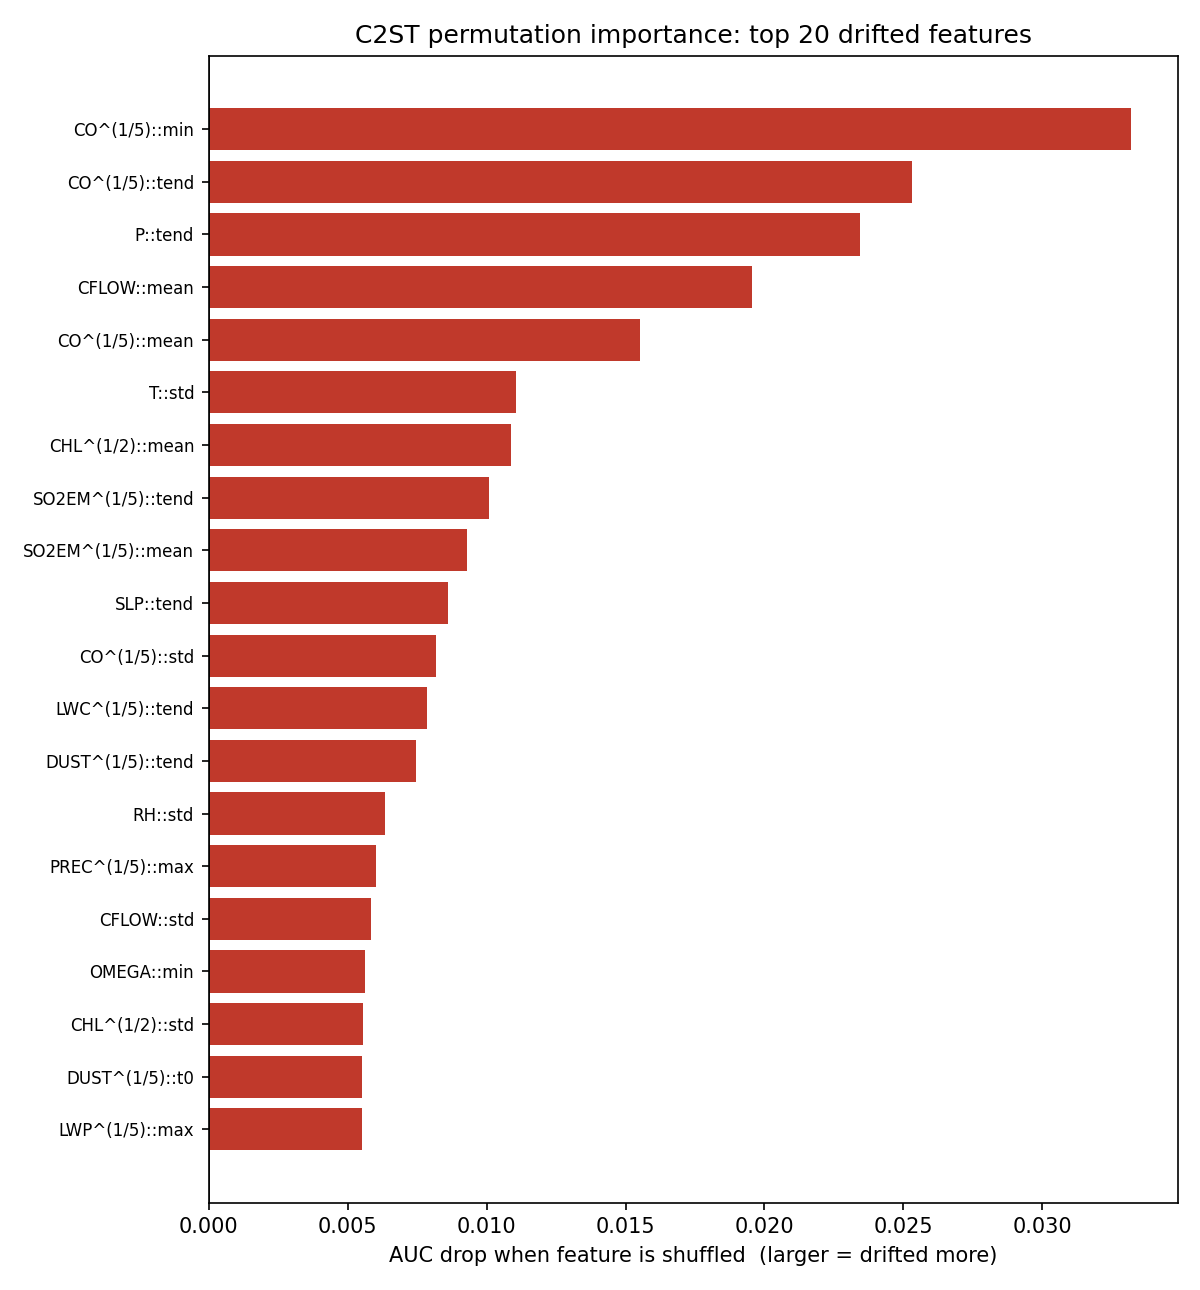
\includegraphics[width=0.80\textwidth]{c2st_feature_importance.png}
\caption{Which channels the classifier used to separate train from test. Longer bar =
that feature drifted more. CO summaries top the list.}
\label{fig:c2st}
\end{figure}

\section*{Shift Test 2 --- MMD permutation test: \emph{is the difference statistically real?}}
\textbf{Intuition.} The MMD test measures how far apart the two groups are, then
shuffles the ``train'' / ``test'' labels thousands of times to see how big that
distance gets when there is genuinely no difference. If the real distance sits far
outside that shuffled range, the difference is real.

\textbf{Result.} Observed \textbf{MMD$^2 = 0.0072$} vs.\ a shuffled null centered at
$0$; \textbf{$p = 0.0008$} (the smallest attainable with 5000 shuffles) and the
observed value sits \textbf{$\sim$7 standard deviations} into the tail
(Figure~\ref{fig:mmd}). An independent energy-distance test agrees ($p = 0.001$).
Caveat: with enough independent episodes \emph{any} nonzero difference becomes
significant, so a tiny $p$ means the shift is \emph{real}, not \emph{large}.

\begin{figure}[H]
\centering
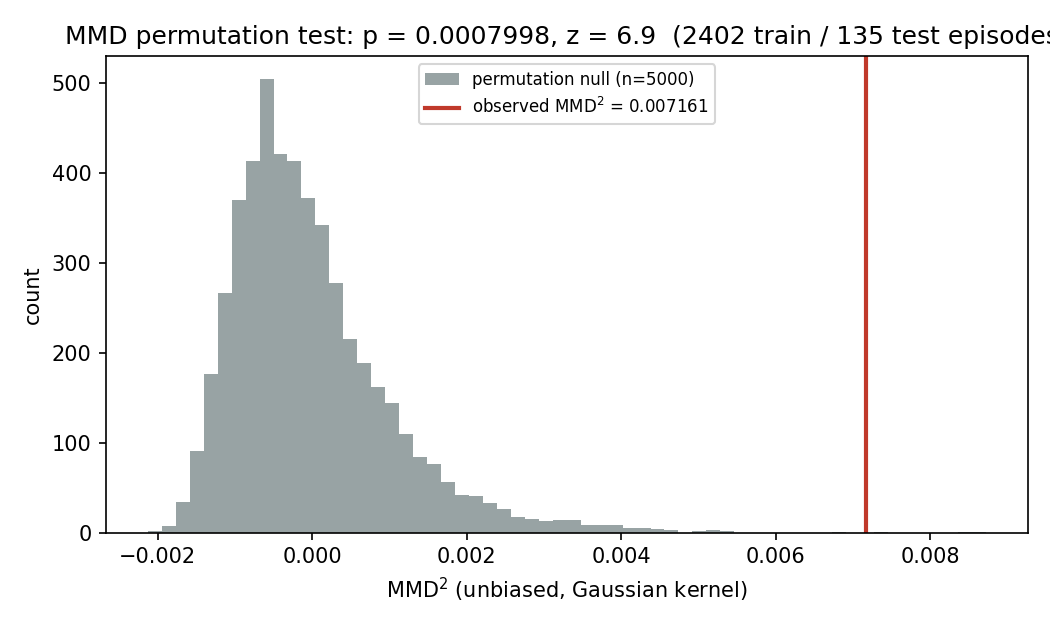
\includegraphics[width=0.68\textwidth]{mmd_null.png}
\caption{Grey = MMD$^2$ under shuffled labels (the ``no difference'' world). Red = the
observed value; it lies far to the right of anything chance produced.}
\label{fig:mmd}
\end{figure}

\section*{Shift Test 3 --- kNN overlap: \emph{does the test still sit inside training territory?}}
\textbf{Intuition.} A difference in \emph{distribution} is not the same as a move into
\emph{new} territory. For each test episode we ask: is there a training episode
nearby? We compare each test point's distance to its nearest training neighbor
against how far training points sit from \emph{each other}.

\textbf{Result.} Median distances are nearly equal --- train$\to$train $8.01$,
test$\to$train $8.36$ (\textbf{ratio 1.04}) --- and only \textbf{7.4\%} of test
episodes fall beyond the training 95th percentile (3.7\% beyond the 99th,
Figure~\ref{fig:knn}). Despite the significant shift, test episodes overwhelmingly
land \emph{inside} the region the models were trained on: \textbf{overlap holds}.

\begin{figure}[H]
\centering
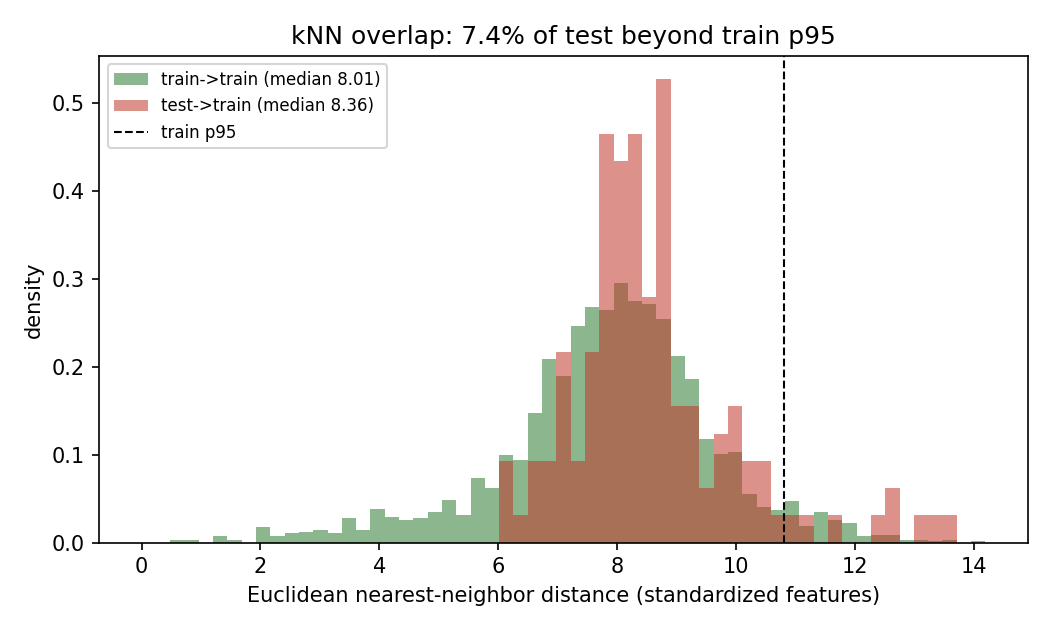
\includegraphics[width=0.68\textwidth]{knn_overlap.png}
\caption{Distance to the nearest \emph{training} episode. Green = training to itself;
red = test to training. They overlap heavily; only a thin red tail crosses the
training 95th-percentile line.}
\label{fig:knn}
\end{figure}

\section*{Shift verdict}
\begin{center}
\begin{tabular}{lll}
\hline
\textbf{Test} & \textbf{Question} & \textbf{Answer} \\
\hline
C2ST & Are train and test different? & Yes --- AUC $0.79$; driven by CO \\
MMD  & Is that difference significant? & Yes --- $p = 0.0008$, $\sim$7$\sigma$ \\
kNN  & Does test stay in training support? & Mostly --- ratio $1.04$, 7.4\% past p95 \\
\hline
\end{tabular}
\end{center}
The test-period weather is \textbf{genuinely and significantly different} (largely a
CO / air-mass-source drift), but the difference is \textbf{modest} and the test
episodes \textbf{stay within the training support}. Because overlap holds, the effect
measured where both models have data (ATT) remains trustworthy, while the
significant-but-real shift is why we prefer ATT over estimands (ATE/ATC) that push the
models onto sparser regions.

\section*{The variables and how they relate}
Beyond the split itself, it helps to see the raw structure of the 22 inputs and the
outcome. Figure~\ref{fig:scatter} is the full pairwise scatter matrix (every variable
against every other; diagonal = each variable's histogram), using one point per sample
(the trajectory mean). Figure~\ref{fig:corr} summarizes the same relationships as
correlations --- \emph{Pearson} (linear) beside \emph{Spearman} (rank/monotonic).

The headline: \textbf{no single dominant driver of CCN}. The strongest correlate is
downwelling solar radiation (\texttt{SWGDN}, $+0.33$), followed by cloud liquid-water
path, low-cloud fraction, and wind speed (all $\approx-0.25$). CCN rises under sunny,
warm, low-cloud, calm conditions and falls with more cloud/rain/wind --- a coherent
``clean-marine'' signature. Pearson and Spearman are nearly identical, so these
\emph{marginal} relationships are close to monotone-linear; the strong nonlinearity is
in the \emph{joint} structure, not the one-to-one marginals. Notably \texttt{CO} --- the
variable that dominates the train/test drift above --- has only a weak marginal
correlation with CCN, consistent with it flagging \emph{when} wildfire air arrives
rather than setting CCN on its own.

\begin{figure}[H]
\centering
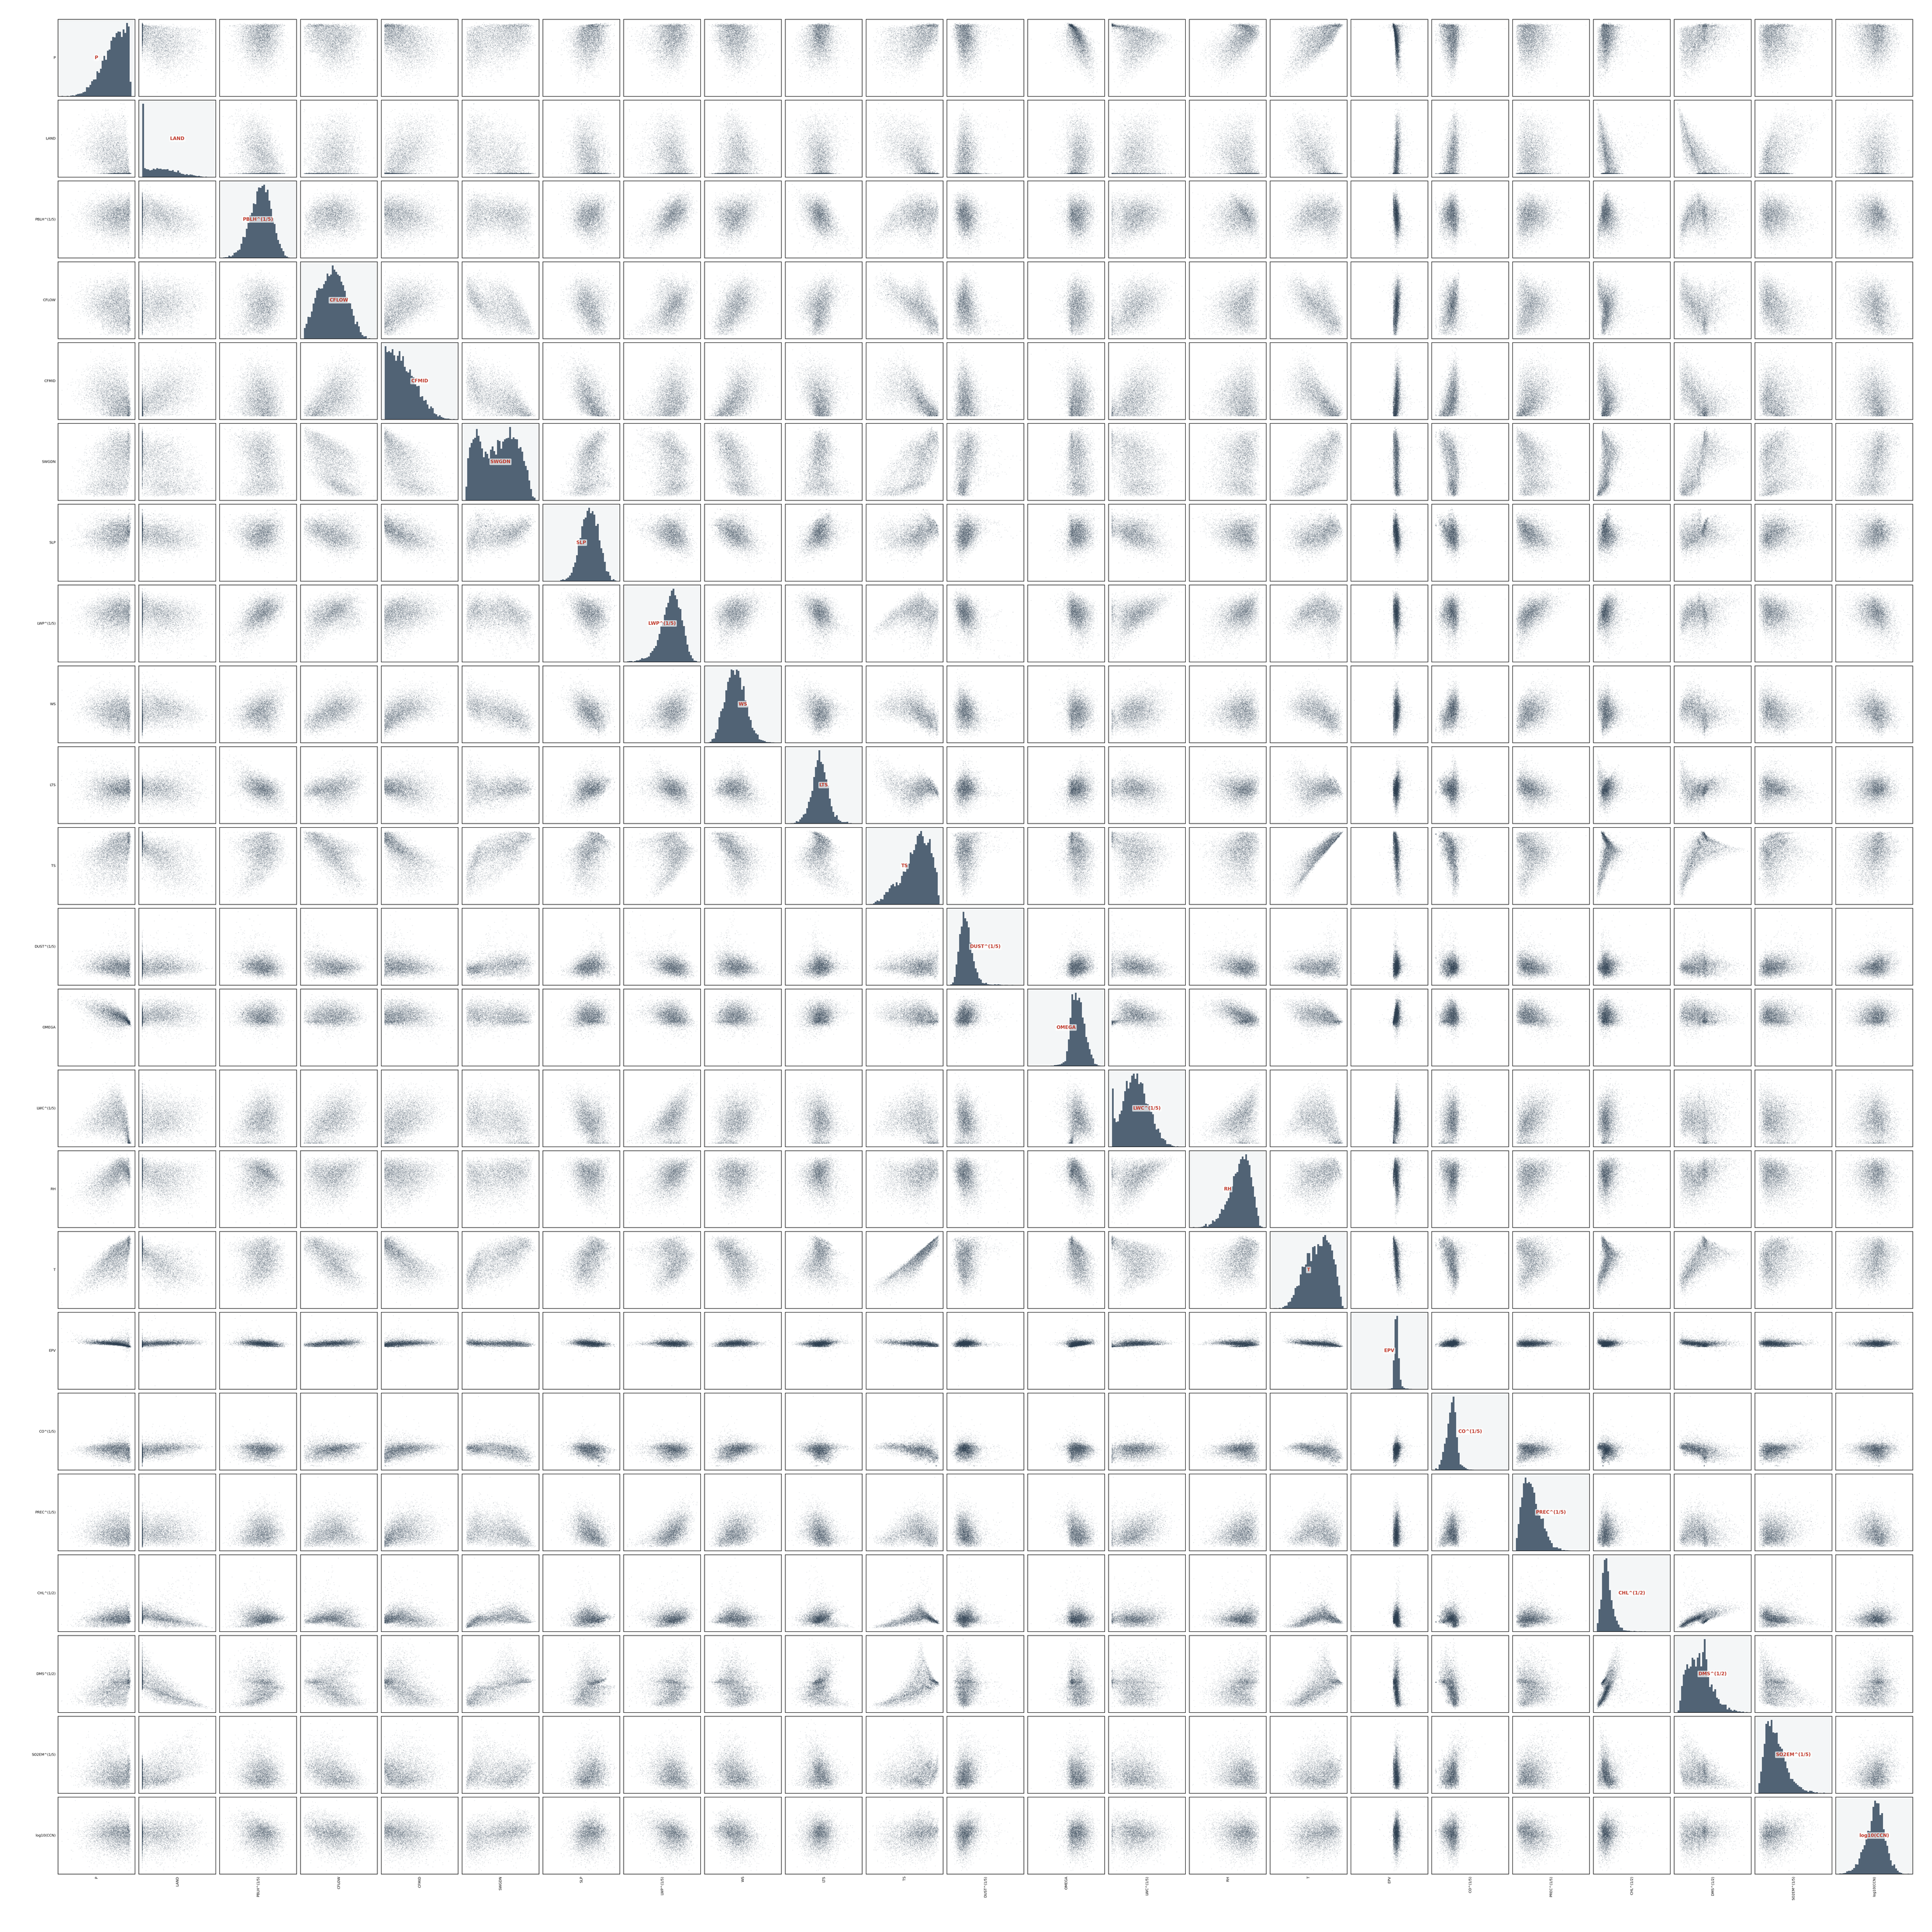
\includegraphics[width=0.72\textwidth]{pairwise_scatter_small.png}
\caption{Pairwise scatter matrix of all 22 channels + \texttt{log10(CCN)} (bottom-right),
6000 samples, per-sample trajectory means. The bottom row / right column shows each
variable against the outcome. (Downscaled here; full-resolution PDF available separately.)}
\label{fig:scatter}
\end{figure}

\begin{figure}[H]
\centering
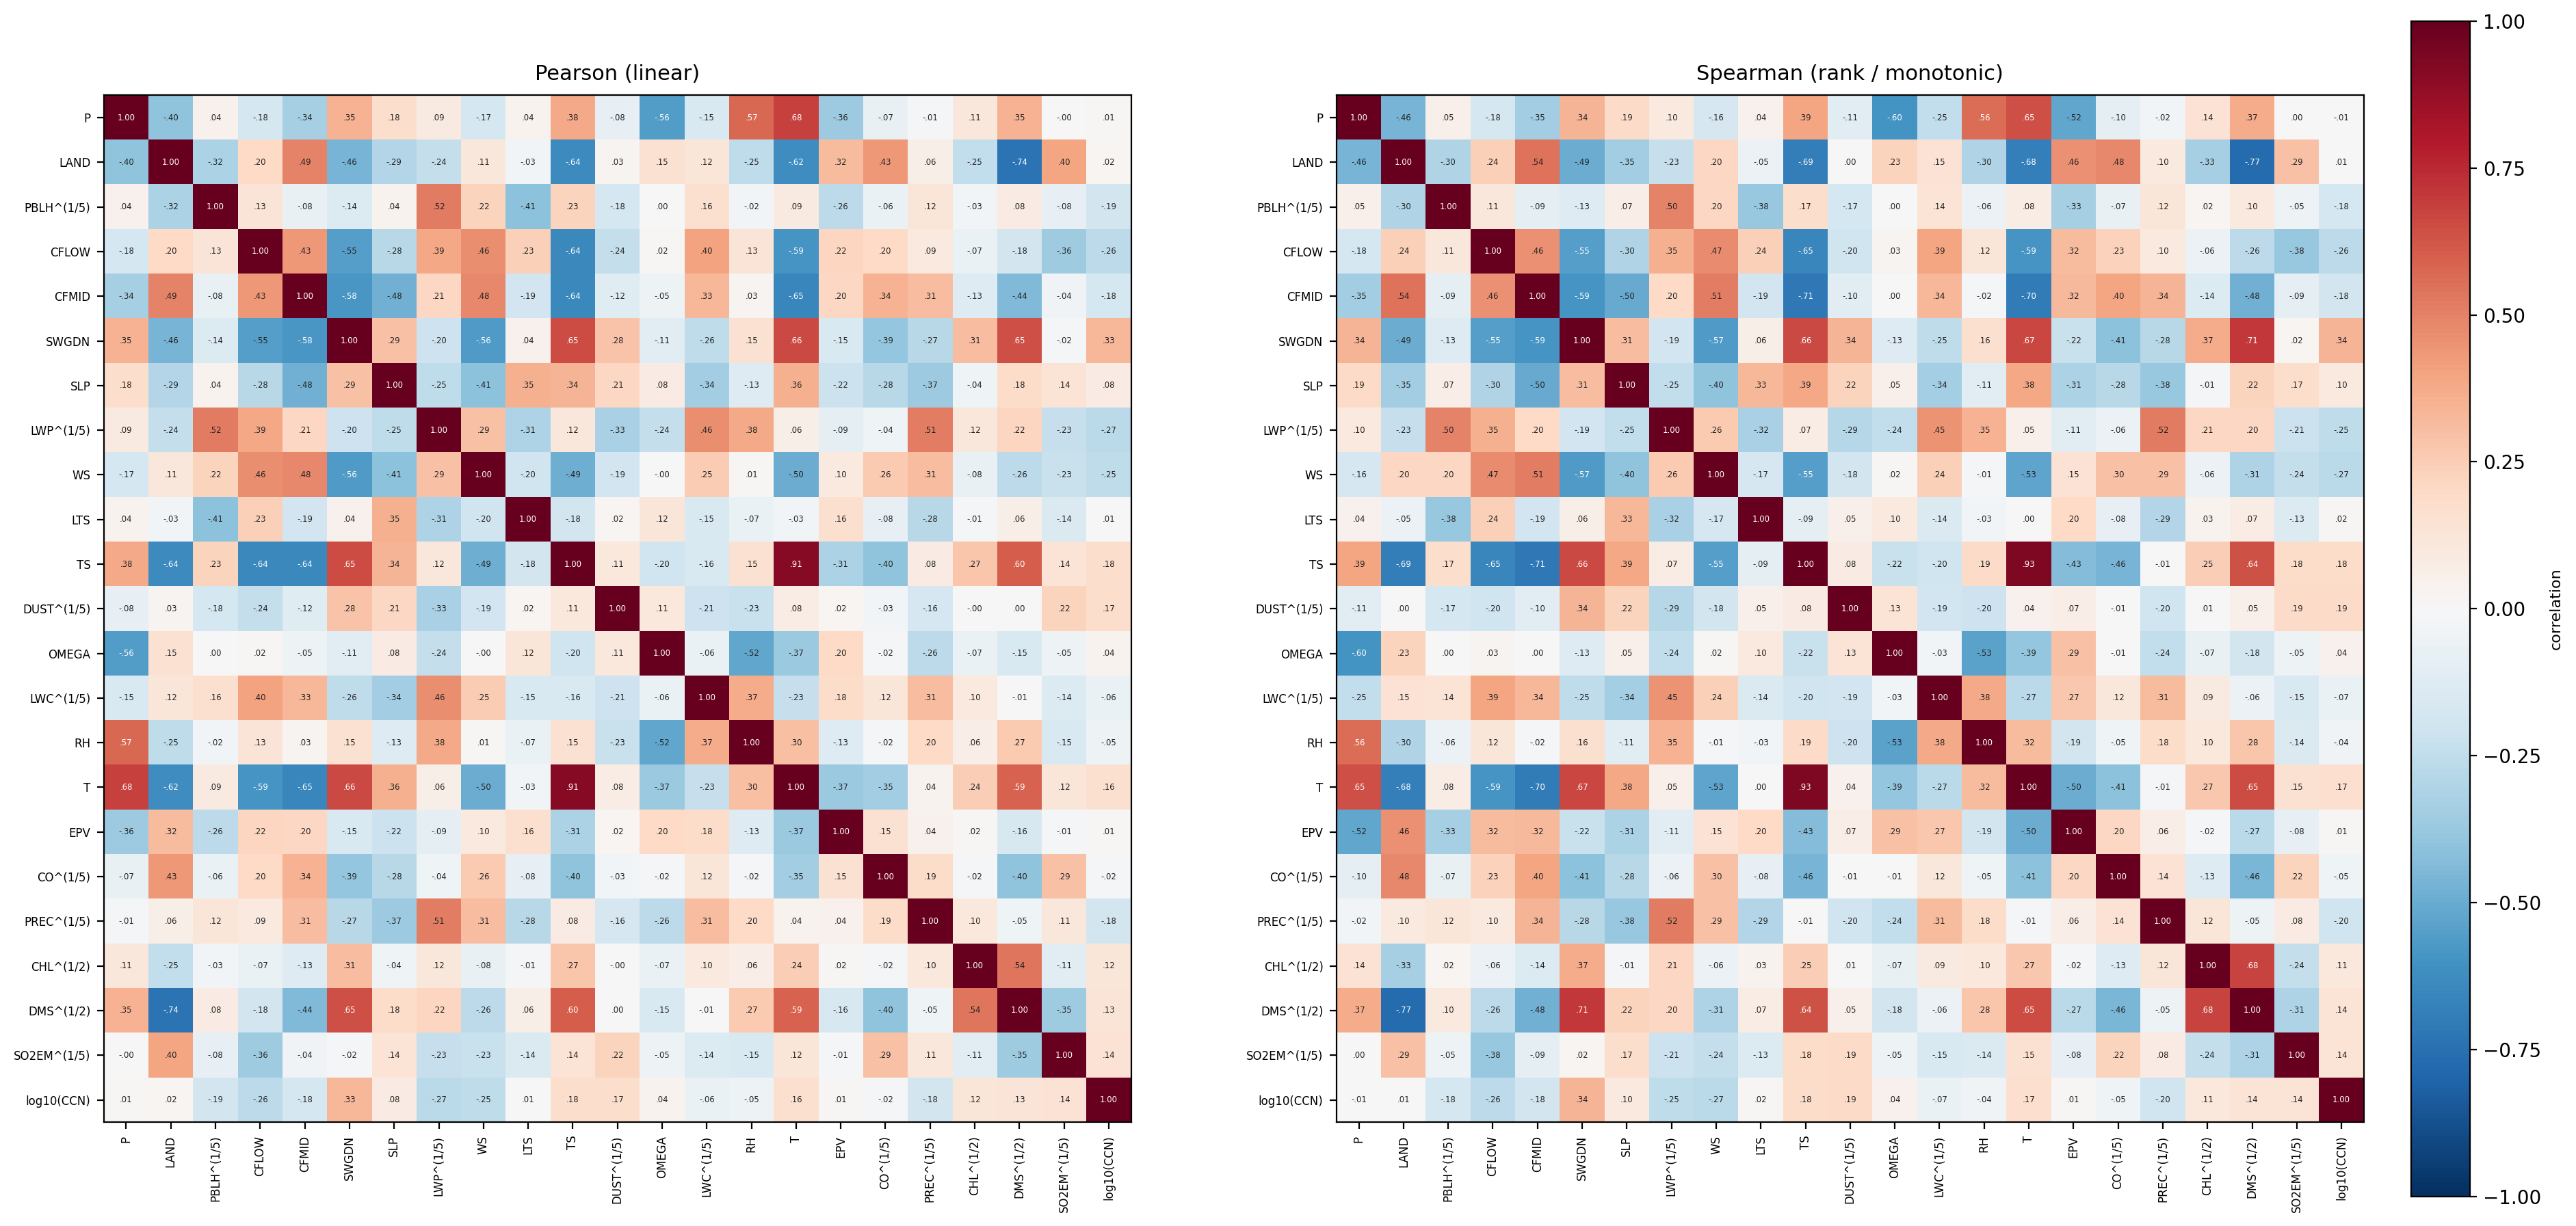
\includegraphics[width=0.95\textwidth]{correlation_heatmap.png}
\caption{Correlation of all 23 variables over 20{,}000 samples (per-sample means).
Left = Pearson (linear), right = Spearman (rank). Red = negative, blue = positive.
Their near-identity indicates the marginal relationships are close to monotone-linear.}
\label{fig:corr}
\end{figure}

\section*{Are the models calibrated? (PIT)}
Finally, a check on the stochastic generators themselves. For each held-out point we
compute the \textbf{PIT} (probability integral transform): the fraction of the model's
predicted samples that fall below the observed CCN. If the predicted distribution is
right, PIT values are uniform, so the histogram should be \textbf{flat}. A
\textbf{U-shape} means the intervals are too narrow (overconfident); a dome means too
wide. Figure~\ref{fig:pit} shows the PIT histogram for all 48 sweep configurations.

Most panels show a mild \textbf{U-shape} --- the models are slightly overconfident
(true CCN lands in the tails a bit more often than a calibrated model would predict) ---
but none are severely miscalibrated, and the better configurations are close to flat.
This is the expected regime for energy-score-trained generators and is worth keeping in
mind when reading interval-based quantities.

\begin{figure}[H]
\centering
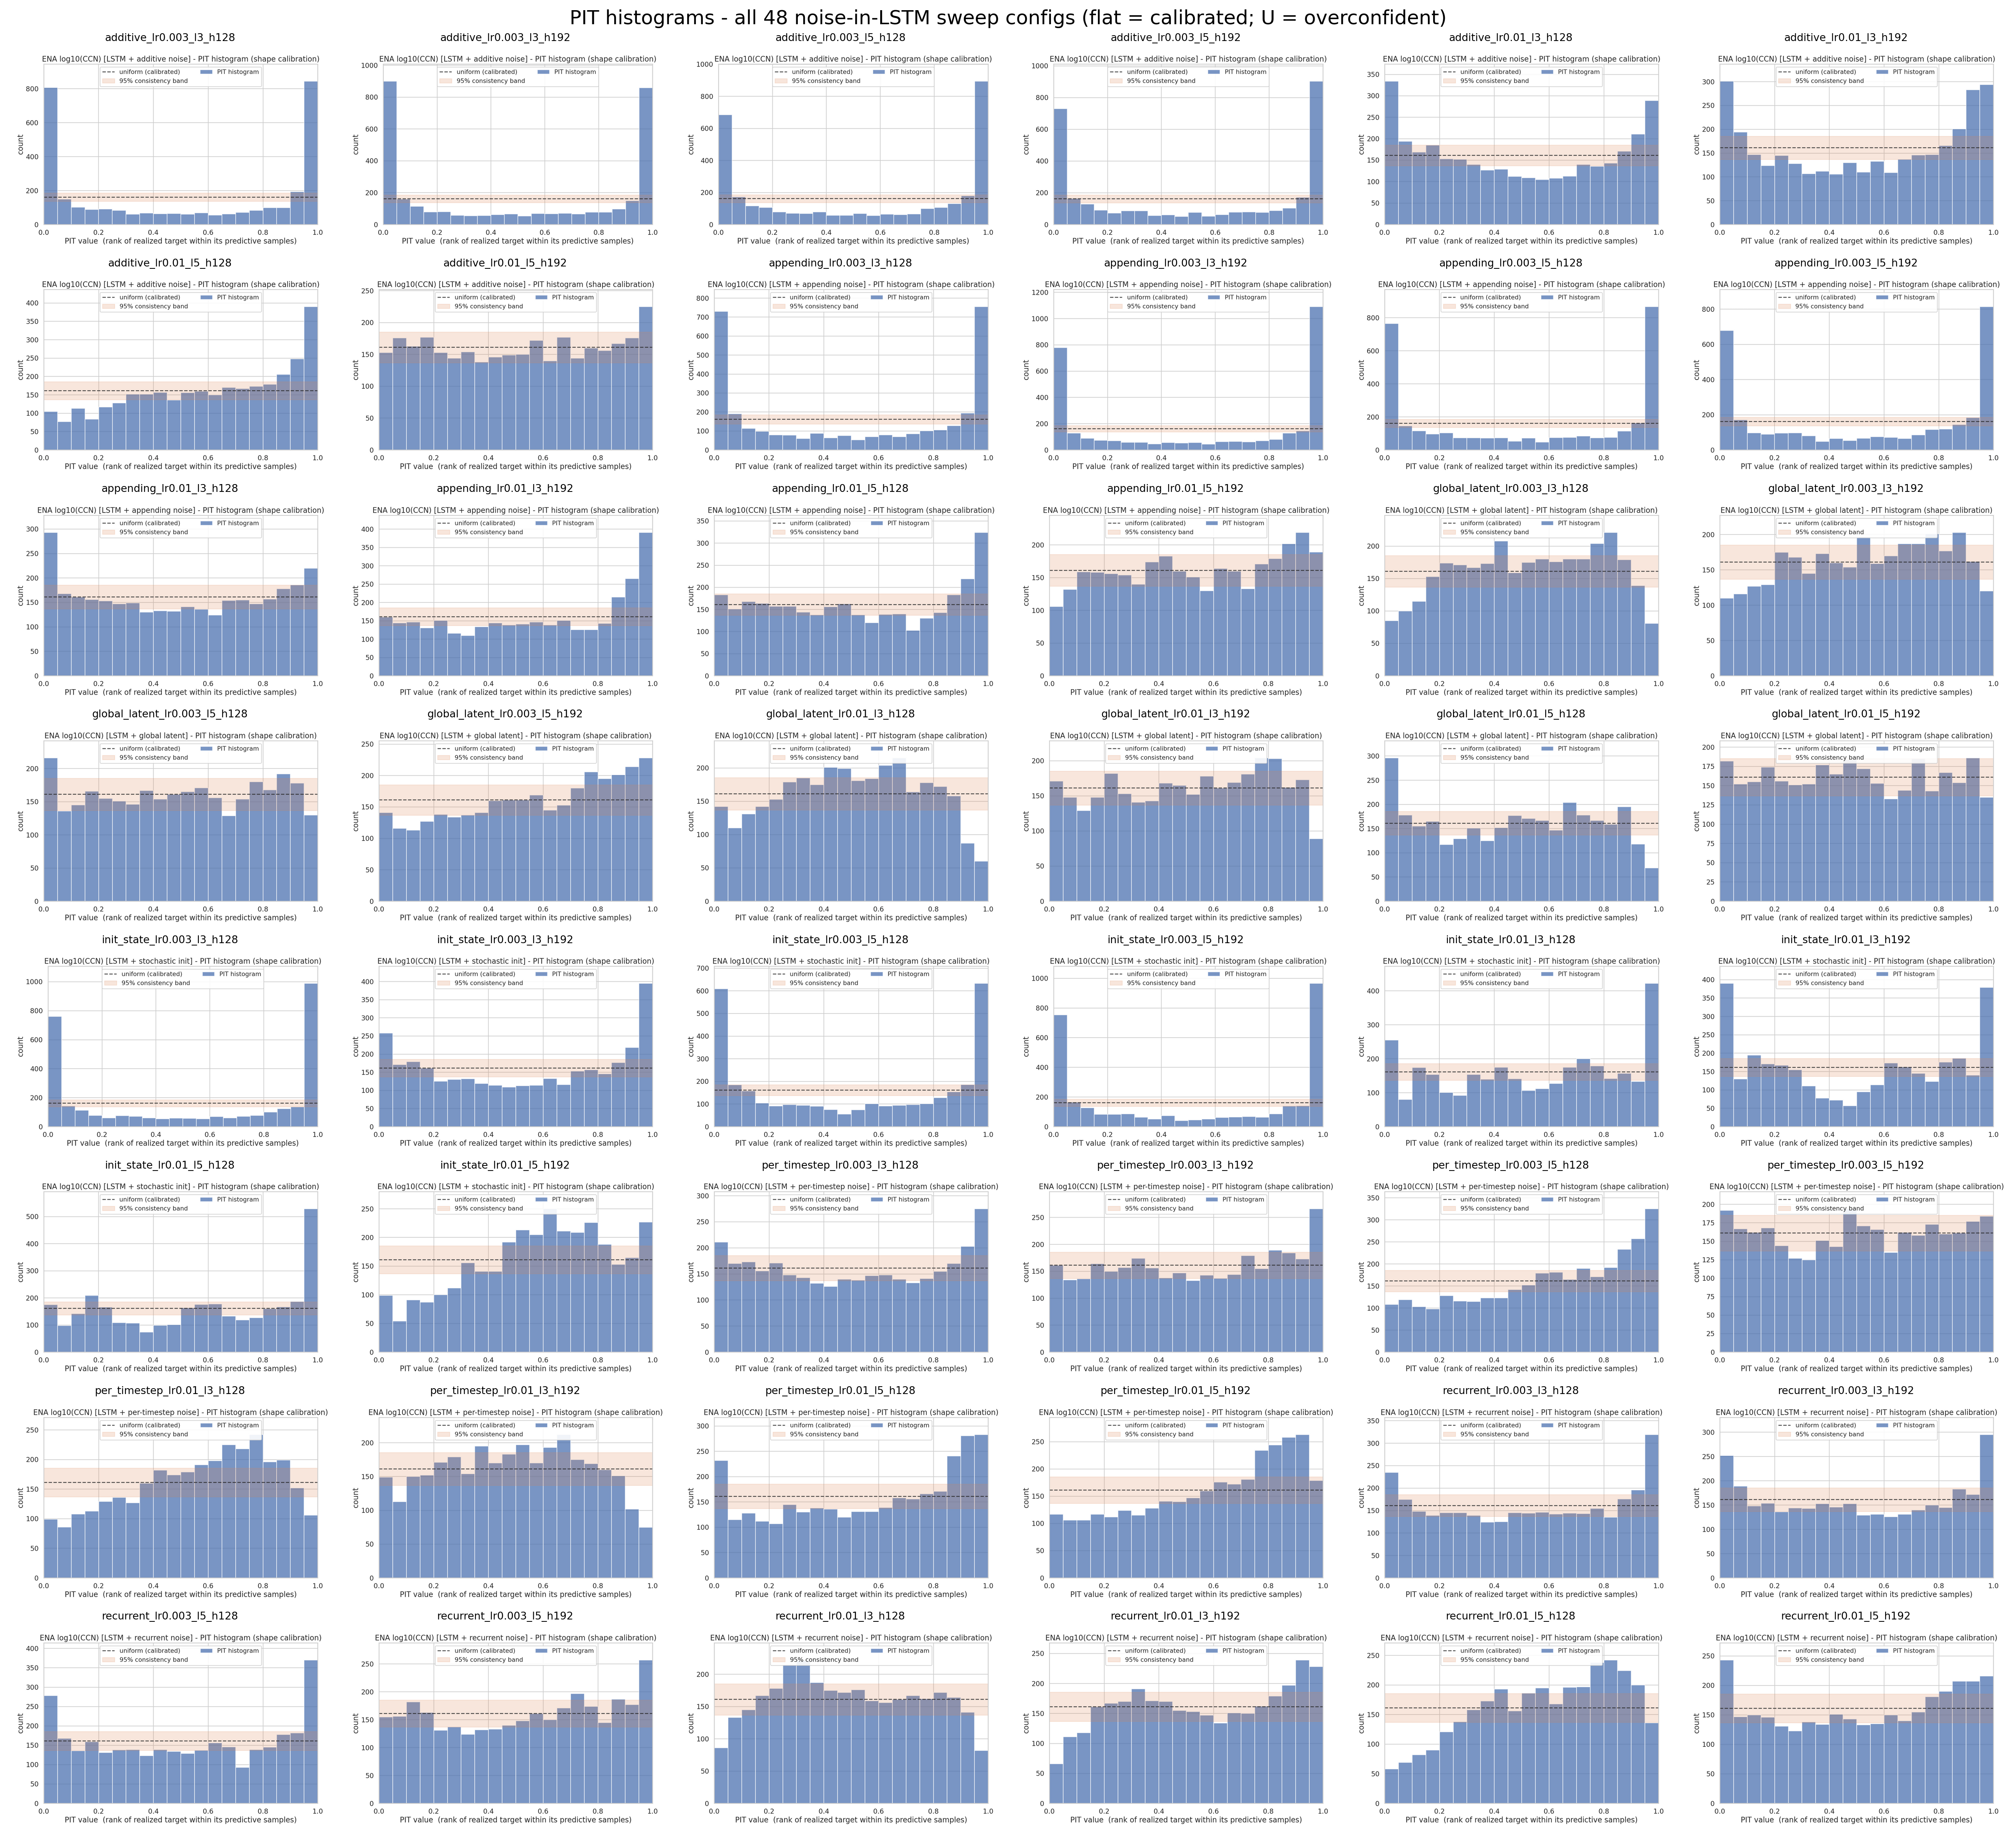
\includegraphics[width=0.95\textwidth]{pit_grid_48.png}
\caption{PIT histograms for all 48 sweep configurations (architecture $\times$
hyper-parameters), each panel titled by its config. Flat = calibrated; U-shape =
overconfident (intervals too narrow); dome = underconfident.}
\label{fig:pit}
\end{figure}

\end{document}
